% ## doc type ----
\documentclass{article}   % article
% \documentclass{beamer}  % slides
% \usetheme{Madrid}

% ## packages ----
\usepackage{hyperref} % url or href
\usepackage{amsmath}  % formulas
\usepackage{graphicx}   % pictures
\usepackage{subcaption} % pictures
\usepackage{float}      % pictures
\usepackage{adigraph}   % graph in computer science
\usepackage{comment}    % comment out lines

\usepackage{tikz}       % Bayesian Network
\usetikzlibrary{bayesnet}

\usepackage{listings}   % codes
\lstset{
  basicstyle=\ttfamily\footnotesize, % Set your code to be drawn with a monospaced font
  breaklines=true, % Enables line breaking
  frame=single % Adds a frame around the code
}

% ## lint ----
% TODO 
\tolerance=10000        
\emergencystretch=\maxdimen
\hyphenpenalty=10000
\hbadness=10000
\usepackage{silence}
\WarningFilter{latex}{Overfull \hbox}
\font\nullfont=cmr10  % remove a warning: Missing character: There is no ; in font nullfont!


% ## cover ----
\title{CIVL 6970 Geometric Design Notes}
\date{2024-02-17}
\author{Michael Chen}


% ## body  ----
\begin{document}
  \pagenumbering{gobble}
  \maketitle
  \newpage
  \pagenumbering{roman}


  % ## index ----
  \tableofcontents
  \newpage


  % ## contents ----




  % ### chapter - HC ----
  \section{Horizontal Curves}

  % ### chapter - VC ----
  \section{Vertical Curves}

  \subsection{Terms} 
  \begin{enumerate}
    \item Centerline - ?
    \item Tangents - 
    \item Vertical curves -
    \item a profile view - ?
    \item grade - + or - ratio, n feet in elevation per 100 feet distance
    
  \end{enumerate}

  \subsection{Goals}
  \begin{enumerate}
    \item constraints of maximum grade and minimum lengths of VCs
    \item conform to the existing terrain
    \item balance earthwork
    \item \underline{avoid} placing the start of a horizontal curve at the \underline{bottom} of a steep grade (due to high speed!)
    \item \underline{ideally}, vertical curves should be located within horizontal curves or on horizontal tangents
  \end{enumerate}


  \subsection{maximum grades - AASHTO Green book 2011}

  \vspace{1cm} % Add 1 centimeter of vertical space
  \begin{center}
  \begin{tabular}{l l}
    \textbf{Road Type} & \textbf{Maximum Grade (\%)} \\
    \hline
    Freeways (based on design speed and terrain) & 3\% to 6\% \\
    Freeways (70 mi/h design speed, level terrain) & 3\% \\
    Interstate System (regardless of terrain) & 4\% \\
    Interstate System (with exception) & Up to 5\% downgrades \\
  \end{tabular}
  \end{center}

  \vspace{1cm} % Add 1 centimeter of vertical space
  \begin{center}
  \begin{tabular}{l l l}
    \textbf{Road Type} & \textbf{Design Speed} & \textbf{Maximum Grade (\%)} \\
    \hline
    Arterials & 60 mi/h or greater (level) & 3\% \\
    Arterials & 40 mi/h (mountainous) & Up to 8\% \\
    Collectors & 70 mi/h (level) & 4\% \\
    Collectors & 20 mi/h (mountainous) & Up to 14\% \\
    Local Roads and Streets & - & Up to 17\% (mountainous terrain) \\
  \end{tabular}
  \end{center}

  \subsection{minimum grade}
  Urban design - min grade is 0.5\%, but 0.3\% may be used

  \newpage

  % ### chapter - ? ----

  % ----------------------------------------
  \section{Writing Formulas}
  \subsection{Equation - ONLY support one formula per line}
  \begin{equation}
    formula 1: f(x) = x^2   ----
    formula 2: \prod_{2}^{n}
  \end{equation}

  \subsection{Align - support MULTIPLE formulas in the same block}
  NOTE: need use package amsmath to enable Align 
  \begin{align*}
    f(x) &= x & 2 \\
    g(x) &= \frac{1}{x} \\
    F(x) = f(x) + g(x) &= \int_{a}^{b} \frac{1}{3}x^3 \\
    W(x) &= \frac{1}{\sqrt{x}} + \frac{1}{\sqrt[3]{y}} \\
    Z(x) &= \left( 3 + 2 \right) * 2
  \end{align*}
  \subsubsection{}
  So which one, align or equation, will you use?


  \subsection{Inline math}
  The form is used for $ f(x) = x^ 2 $ or $\lambda$, so you can easily to use them. 
  https://github.com/LucaCappelletti94/adigraph
  \subsection{Matrics}
  $
  \left[
  \begin{matrix}
    3 & 2 \\
    9 & 4 & x
  \end{matrix}
  \right]
  $

  \newpage


  % ----------------------------------------
  \section{Embedding Pictures/Figures}

  \subsection{One figure}
  NOTE: need to use package graphicshttps://github.com/LucaCappelletti94/adigraph to enable figure

  \iffalse
  \begin{figure}[h!]
    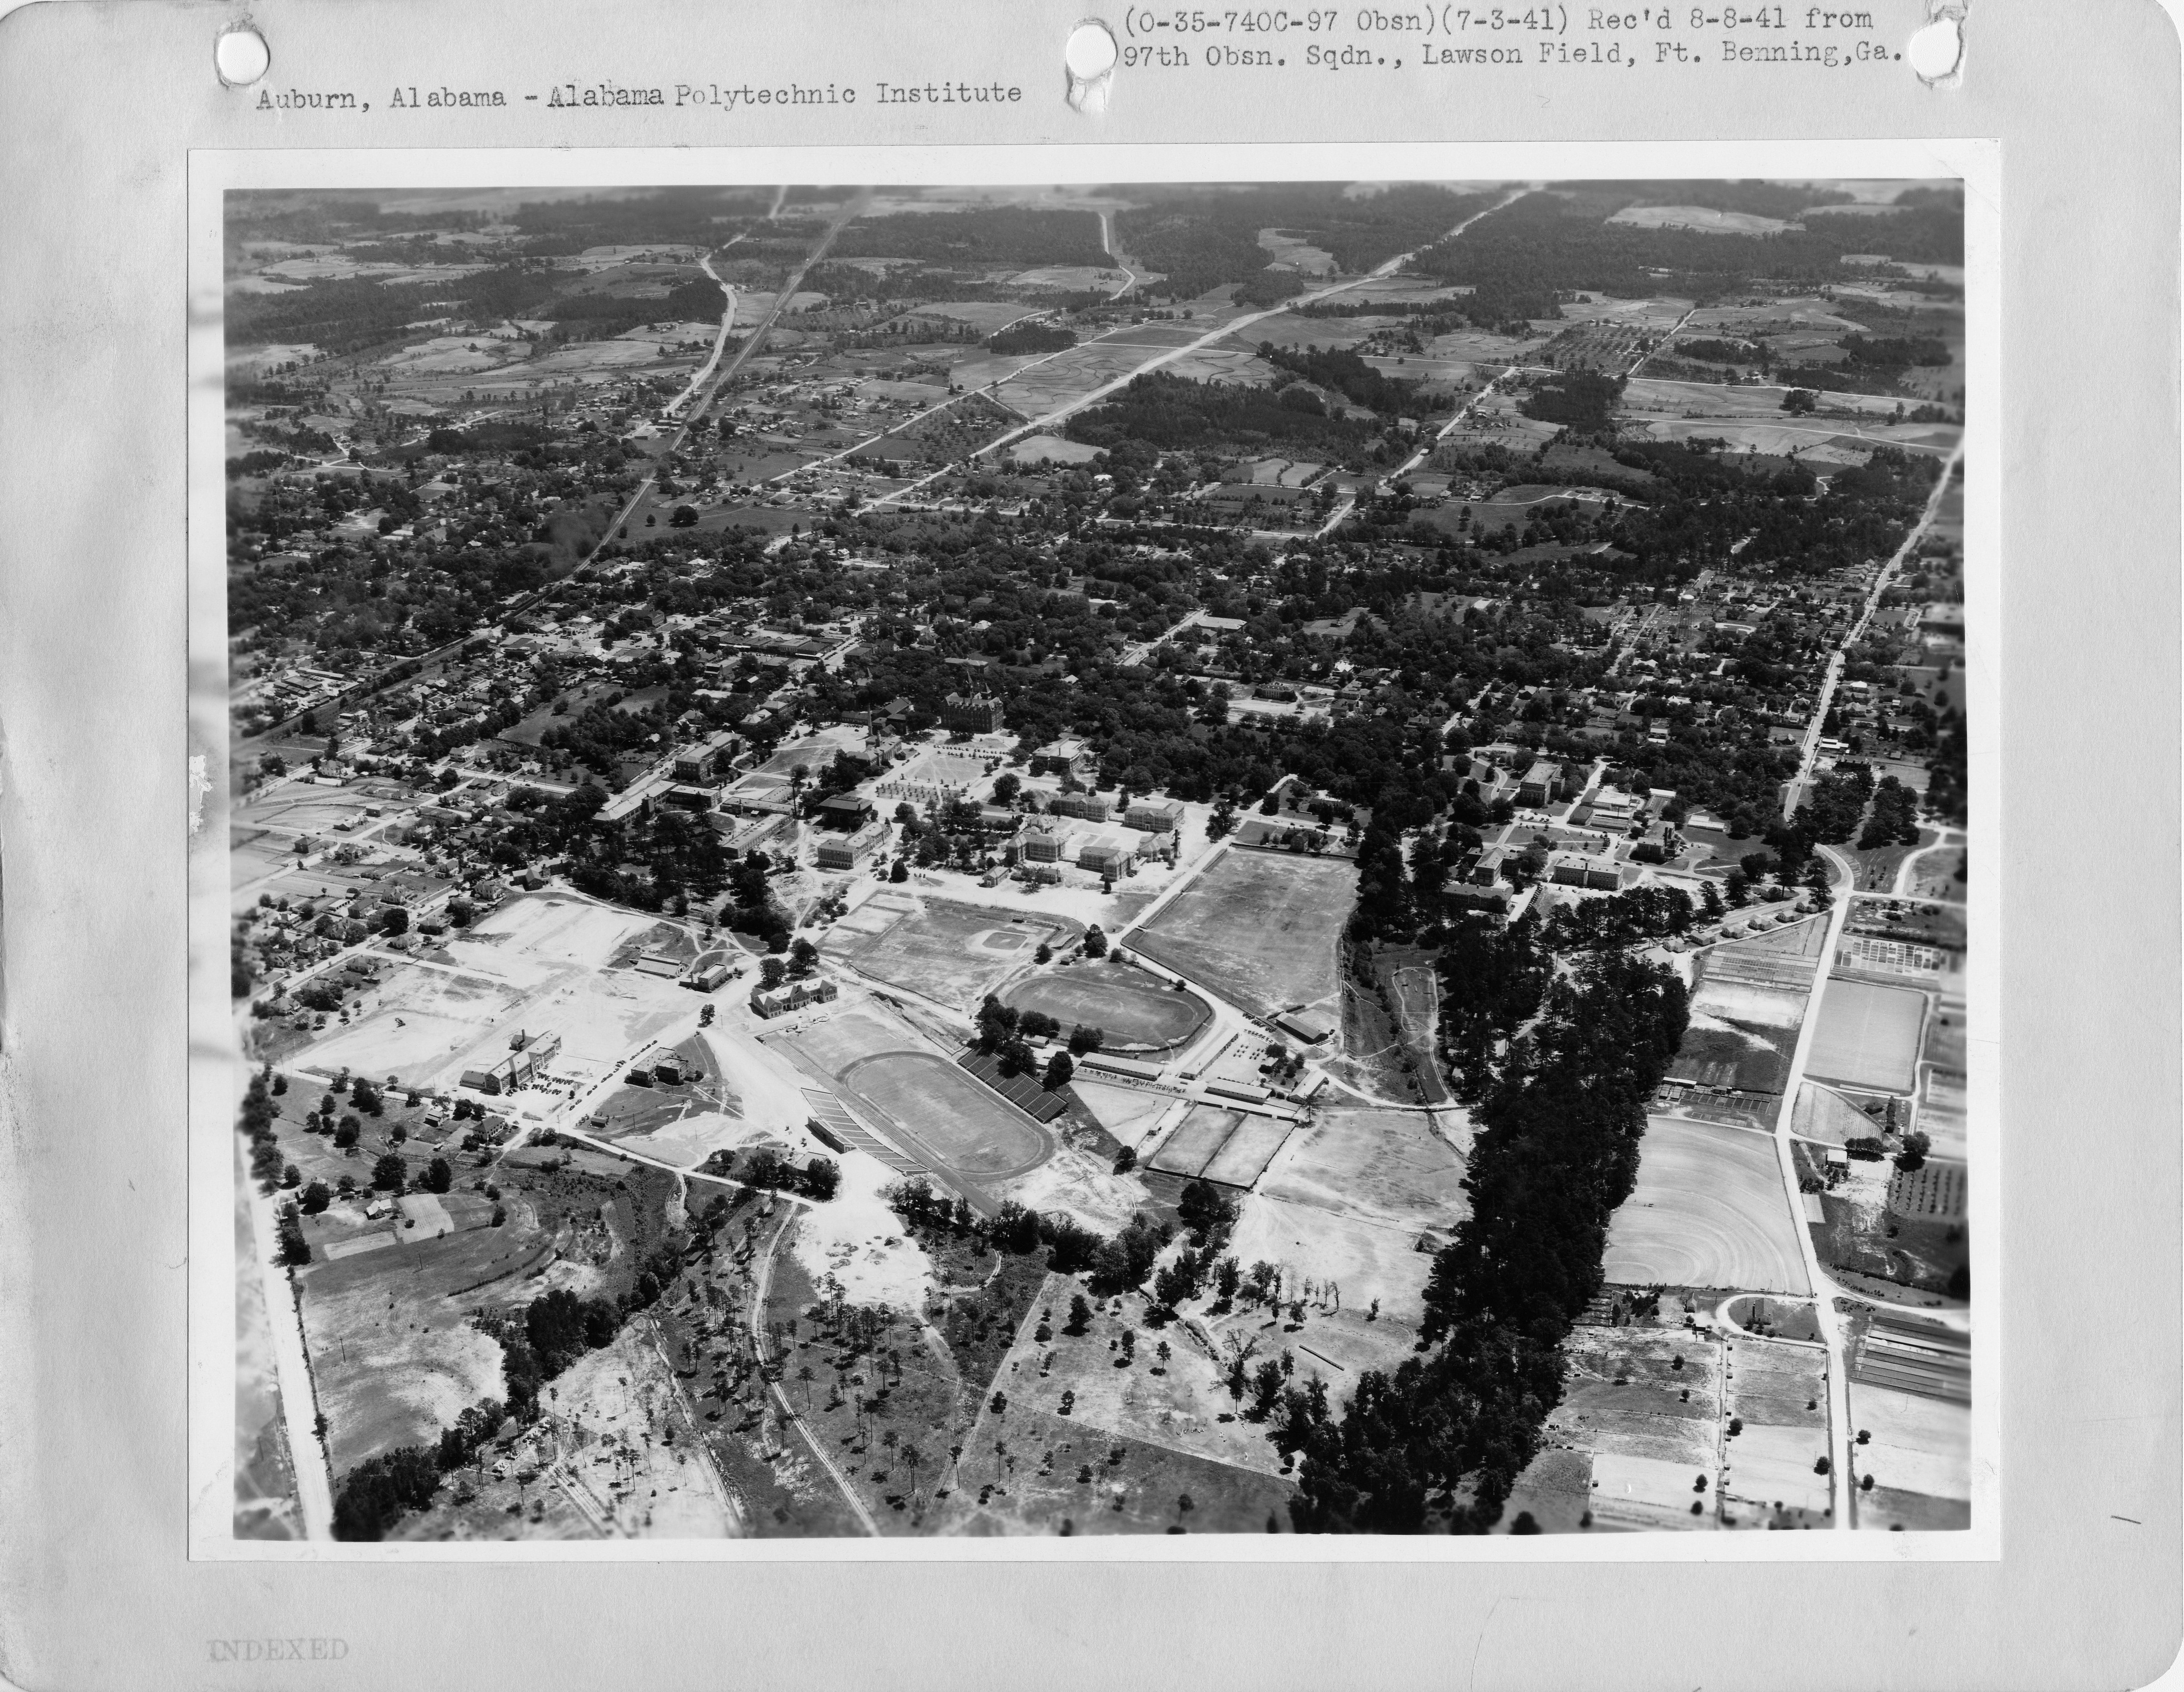
\includegraphics[width=\linewidth]{auburn_01.jpg}
    \caption{Auburn Campus}
    \label{fig:au01}
  \end{figure}

  \subsection{Multiple figures}
  NOTE: need to use package subcaption to enable Multiple figures.
  Here are figures:
  \begin{figure}[H]
    \centering
    \begin{subfigure}[b]{0.4\linewidth}
      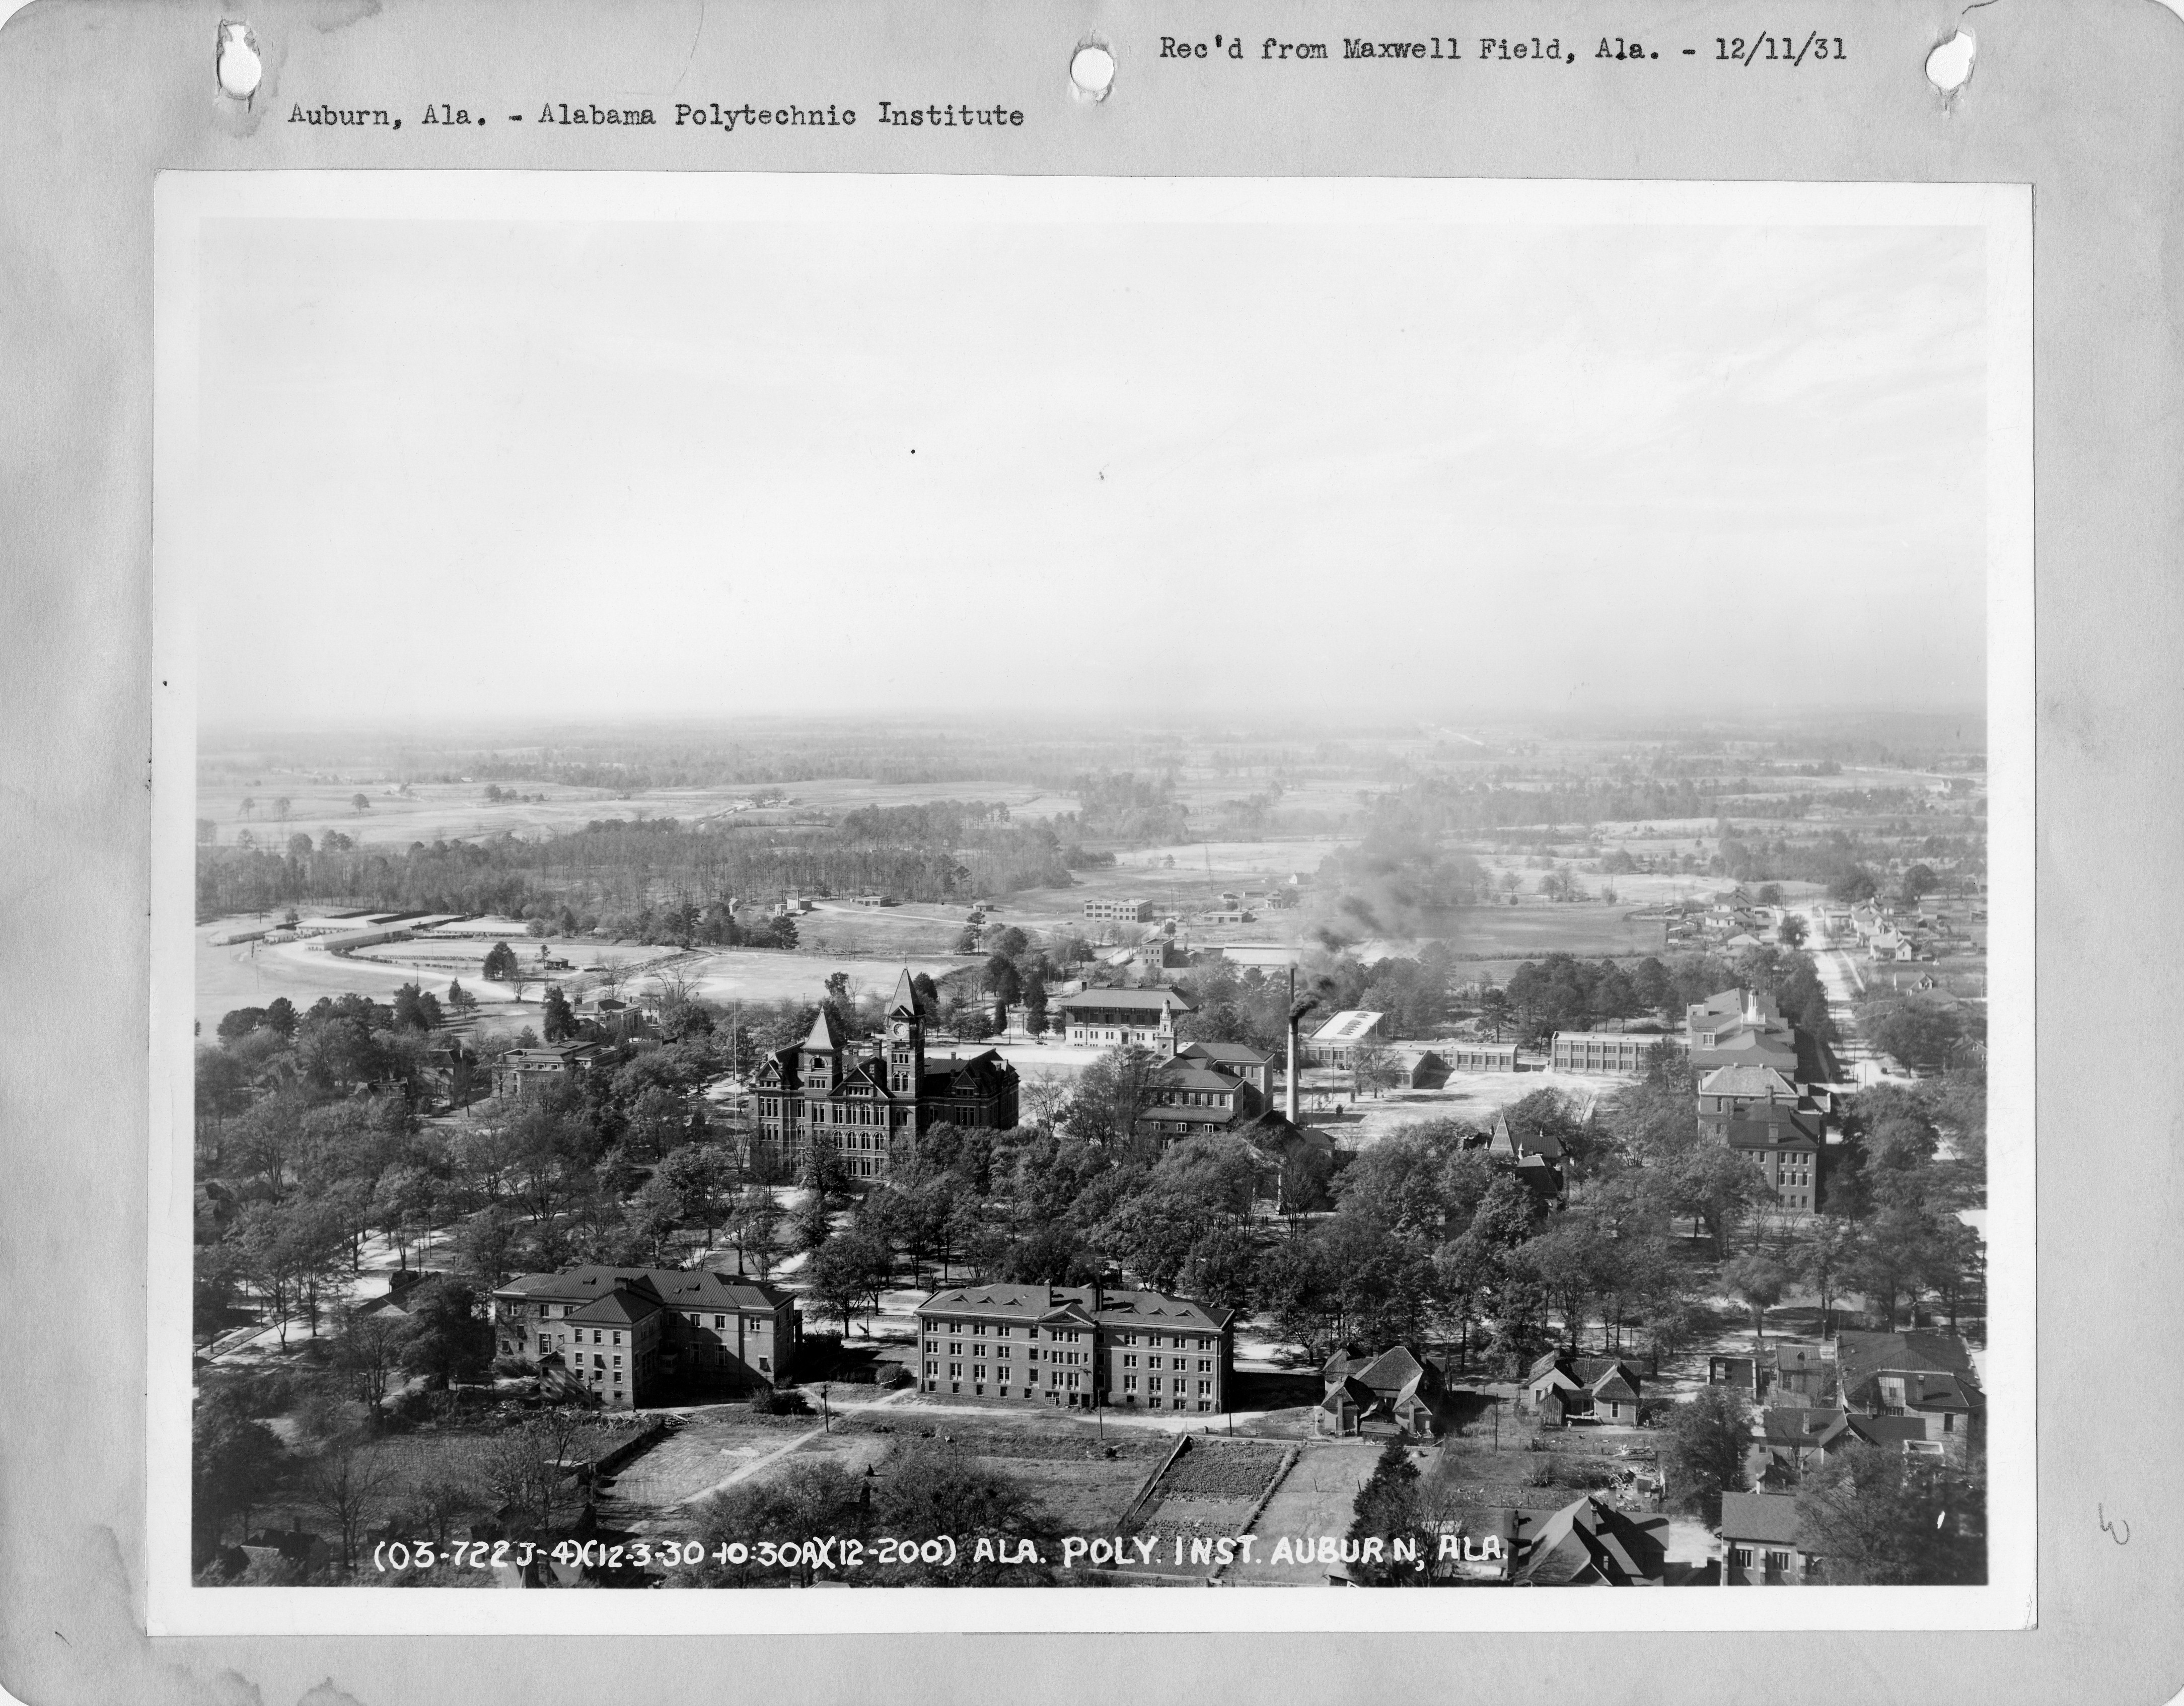
\includegraphics[width=\linewidth]{auburn_02.jpg}
      \caption{Auburn Overview}
    \end{subfigure}
    \begin{subfigure}[b]{0.4\linewidth}
      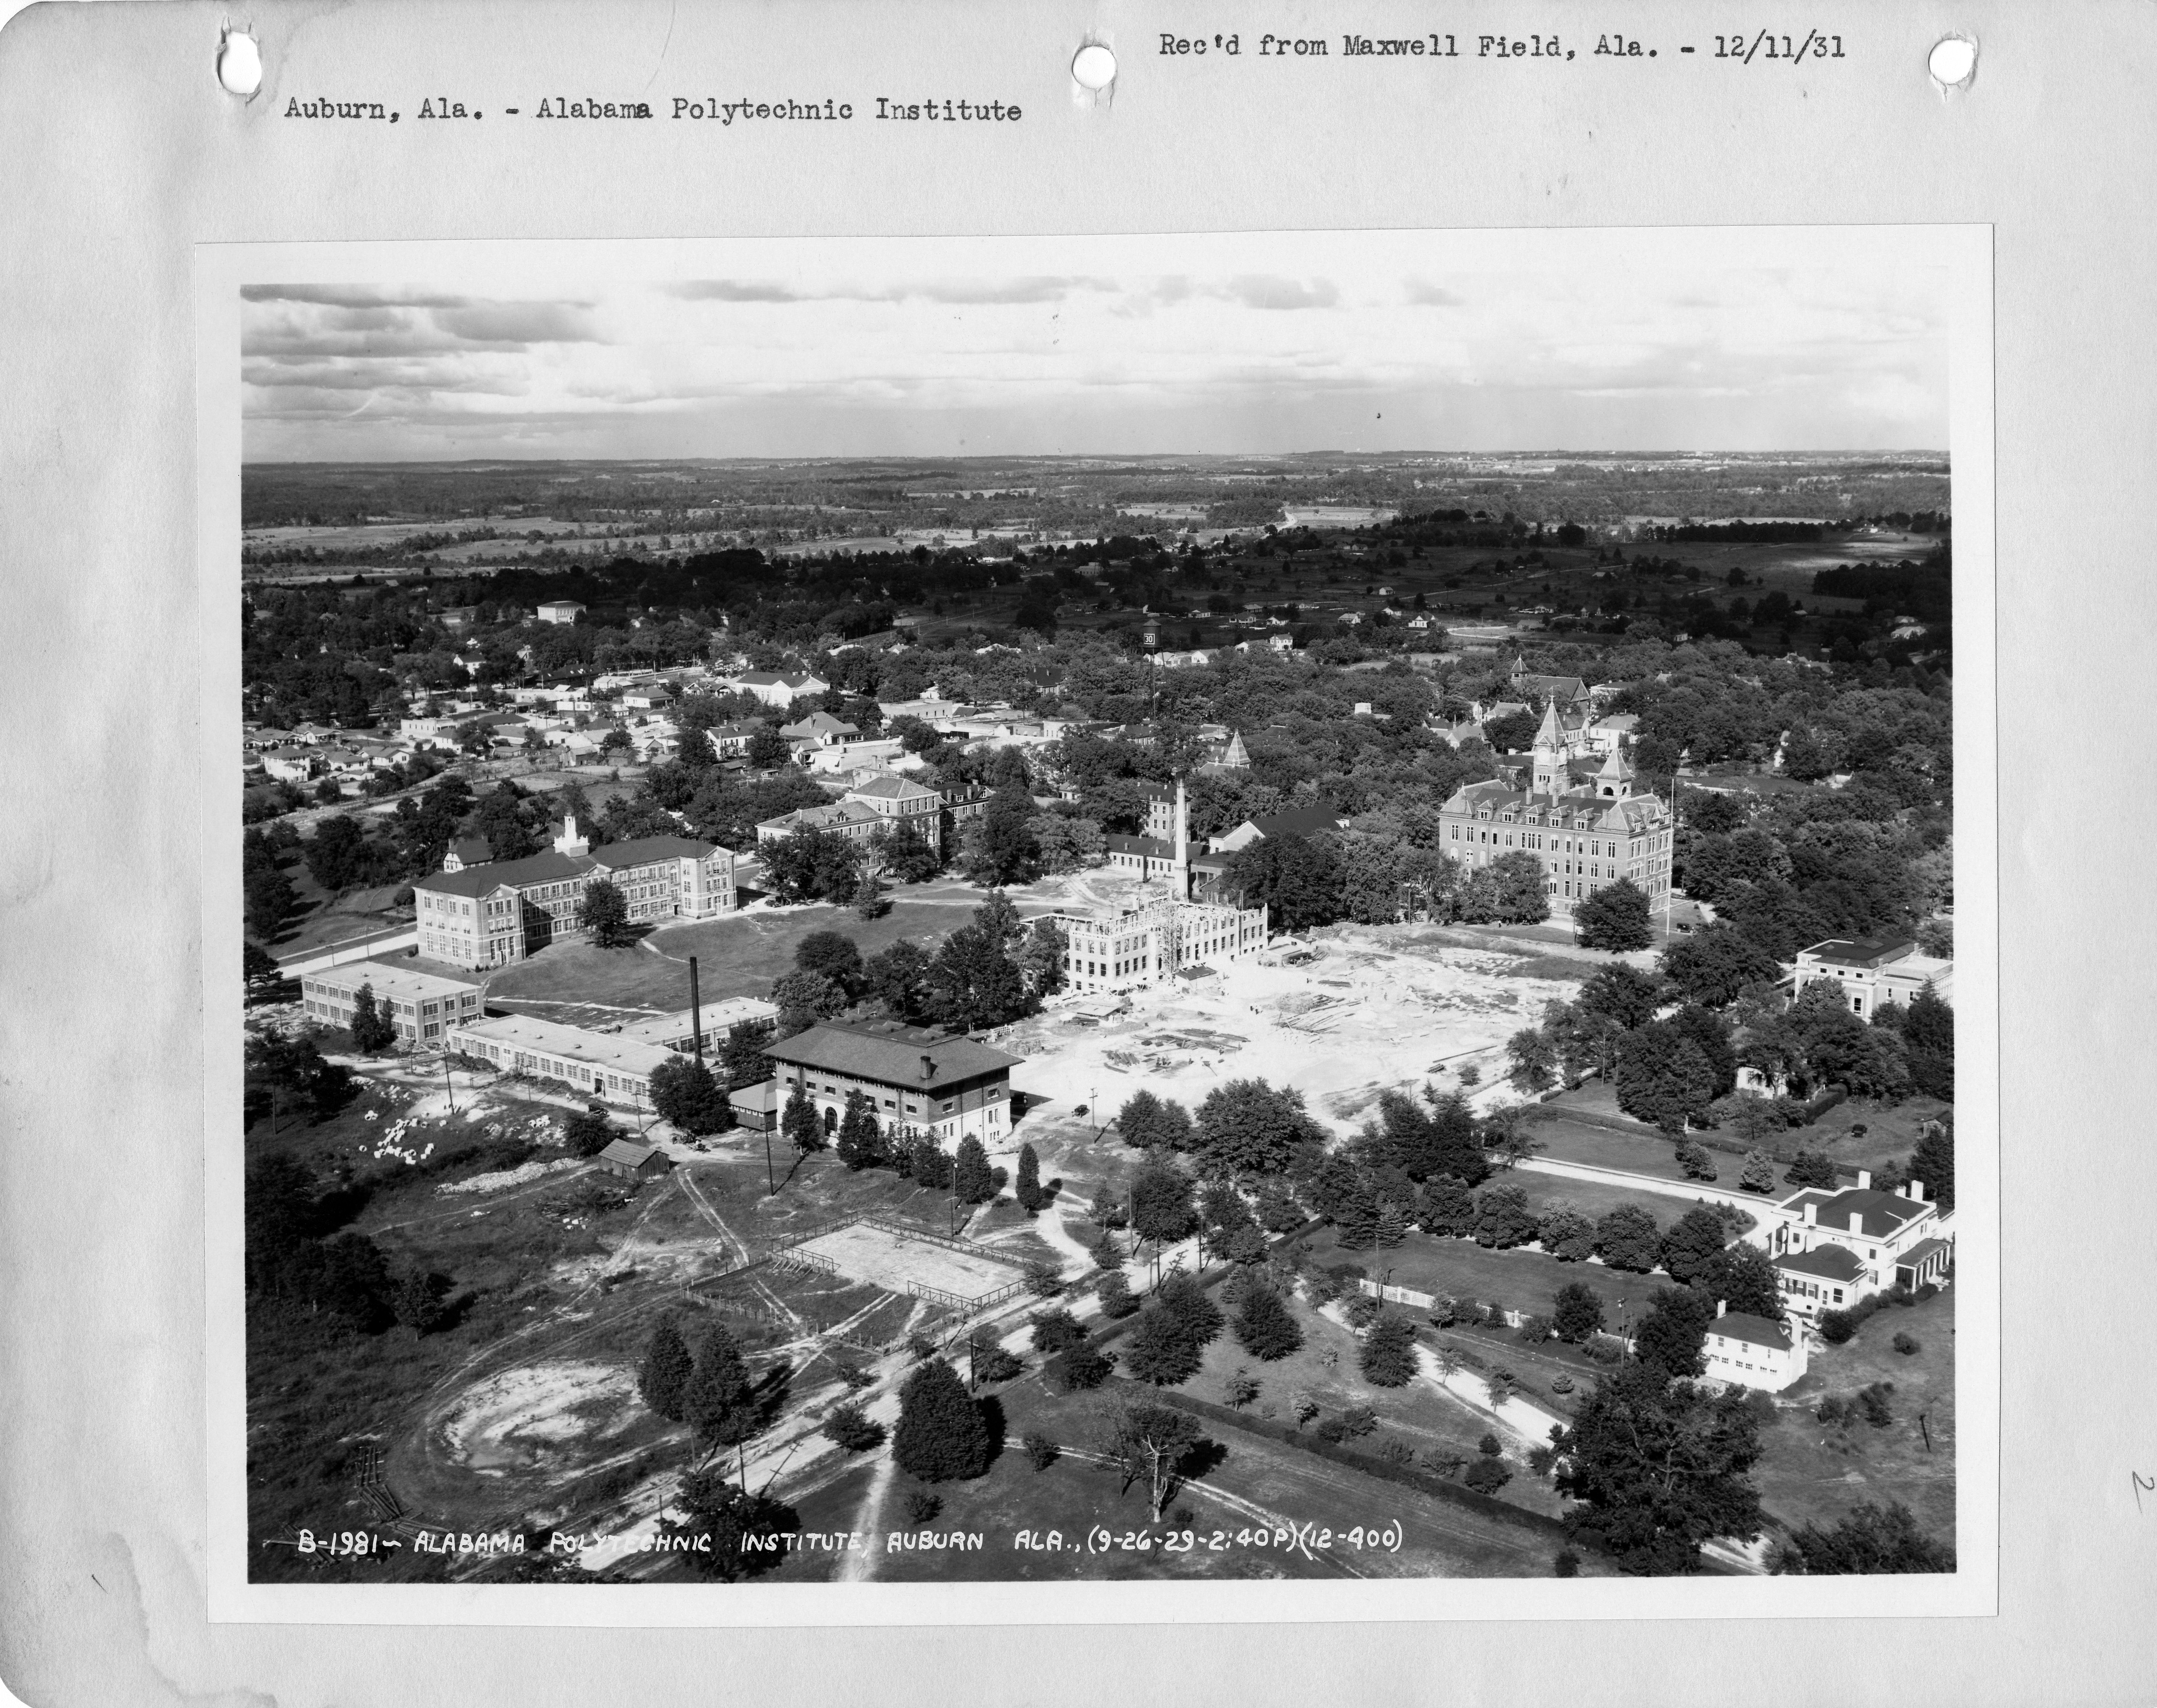
\includegraphics[width=\linewidth]{auburn_03.jpg}
      \caption{Auburn Buildings}
    \end{subfigure}
    \caption{Two Auburn Old Pictures}
    \label{fig:twoPic}
  \end{figure}
  \fi

  \subsection{Use float and H}
  Use package float and attribute H to strictly fix the pictures' posisiton to HERE.

  \begin{lstlisting}[caption={An Example}]
    \usepackage{float}
    ...


    \begin{figure}[H]
      ....
    \end{figure}

    
  \end{lstlisting}
  \newpage


  % ----------------------------------------

  \section{Drawing Bayesian Network and Graph}
  \subsection{Use pagckages: tikz and bayesnet}
  Use 2 packages: tikz and bayesnet to draw Bayesian Network chat.
  \break

  Type 1:
  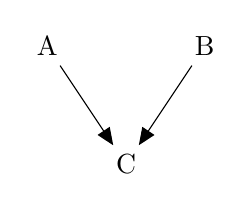
\begin{tikzpicture}
  \node (A) at (0,0) {A};
  \node (B) at (2,0) {B};
  \node (C) at (1,-1.5) {C};
  \draw[->] (A) -- (C);
  \draw[->] (B) -- (C);
  \end{tikzpicture}


  Type 2:
  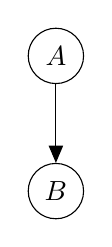
\begin{tikzpicture}
  \node[latent] (A) {$A$};
  \node[latent, below = of A] (B) {$B$};
  \edge {A} {B};
  \end{tikzpicture}
  \iffalse
  \fi
  
 
  \subsection{Use pagckages: adigraph}

  \NewAdigraph{myAdigraph}{
    s:0,0;
    1:2,2;
    3:2,-2;
    2:6,2;
    4:6,-2;
    t:8,0;
}{
    s,1:25;
    s,3:25;
    3,4:25;
    1,2:35;
    2,t:20;
    4,t:30;
    3,1:10;
    4,2:10;
    2,3:15::near start;
    4,1:5::near start;
}
\myAdigraph{}

\newpage


% --------------------------------------
\section{Using packages}
Packages are like plugins to extend the Latex' capabilities. Some common commands are listed here.

\begin{lstlisting}[language=bash, caption={tlmgr commands and etc}]
tlmgr list --only-installed   # show installed packages

tlmgr search <package-name>   # search a packages
tlmgr info <package-name>     # show a package's intro, no matter installed or not
tlmgr install <package-name>  # install a new packages

tlmgr update --self --all     # update package index

kpsewhich article.sty         # locate a package's .sty file

# env variables can define additional directories to be searched. 
echo $TEXMFHOME $TEXMFLOCAL $TEXMFSYSCONFIG 
\end{lstlisting}
\newpage


% --------------------------------------
\section{Generate Slides}
Use the package beamer to generate a pdf file of slides from an article


\begin{lstlisting}[caption={Changes in .tex file}]
  % \documentclass{article}
  \documentclass{beamer}
  \usetheme{Madrid}
\end{lstlisting}

% --------------------------------------
\end{document}